\documentclass[8pt,dvipsnames]{beamer}

\mode<presentation> 
%{ \usetheme[nat,dogma]{Frederiksberg} }

% \usepackage[danish]{babel}
\usepackage{etex}
\usepackage[latin1]{inputenc}
%\usepackage{times}
\usepackage{mathrsfs}
\usepackage[T1]{fontenc}
\usepackage[english]{babel}
\usepackage{hyperref}
\usepackage{animate}
%\usepackage{multimedia}
\usepackage{francois-preamble}
\usepackage{multirow}
\usepackage{cancel}
\usepackage{multirow}
\usepackage{tikz}
\usepackage{manfnt}
\usepackage{framed}


\makeatletter
\newcommand\mathcircled[1]{%
  \mathpalette\@mathcircled{#1}%
}
\newcommand\@mathcircled[2]{%
  \tikz[baseline=(math.base)] \node[draw,circle,inner sep=1pt] (math) {$\m@th#1#2$};%
}
\makeatother





%\usepackage{movie15}

\newcommand{\cc}{{c\!\!,}}
\newcommand{\degr}[1]{{{#1}^\circ}}

\title{Vision and Image Processing:\\ Very Brief Recall on Derivatives}

\author[F.~Lauze] % (optional, use only with lots of authors)
{Fran{\c c}ois Lauze}

\institute[DIKU] % (optional, but mostly needed)
{
  Department of Computer Science\\
  University of Copenhagen
}

\date[2020-21 B2]{VIP, 2.11.2020}


\definecolor{gold}{rgb}{0.95,0.83,0.0}
\definecolor{orange}{rgb}{0.95,0.7,0.0}
% \definecolor{backblue}{rgb}{0.93,0.94,0.99}
\definecolor{backblue}{rgb}{0.95,0.94,0.99}
\setbeamercolor*{background canvas}{bg=backblue} 



\newcommand{\myemph}[1]{{\color{blue}{#1}}}
\newcommand{\intrg}[1]{\int_{{#1}=-\infty}^\infty}
\newcommand{\intRR}{\int_{-\infty}^\infty}
\newcommand{\numpy}{\texttt{numpy}}

\AtBeginSection[]
{
  \begin{frame}<beamer>{Outline}
    \tableofcontents[currentsection,currentsubsection]
  \end{frame}
}

\begin{document}
\maketitle


%-------------------------------------------------------------------
%   Start slides
%-------------------------------------------------------------------




%----------------------------------------------

 
  
% \end{frame}

\begin{frame}
  \frametitle{Plan for this lecture}
  \begin{itemize}
  \item Derivatives in 1D
  \item Derivatives in 2D/3D, Gradients
  \end{itemize}
\end{frame}


\section{Derivatives in 1D}

\begin{frame}{Secants, limits and derivatives}
  \begin{overprint}   
      \onslide<1>
        \begin{center}
          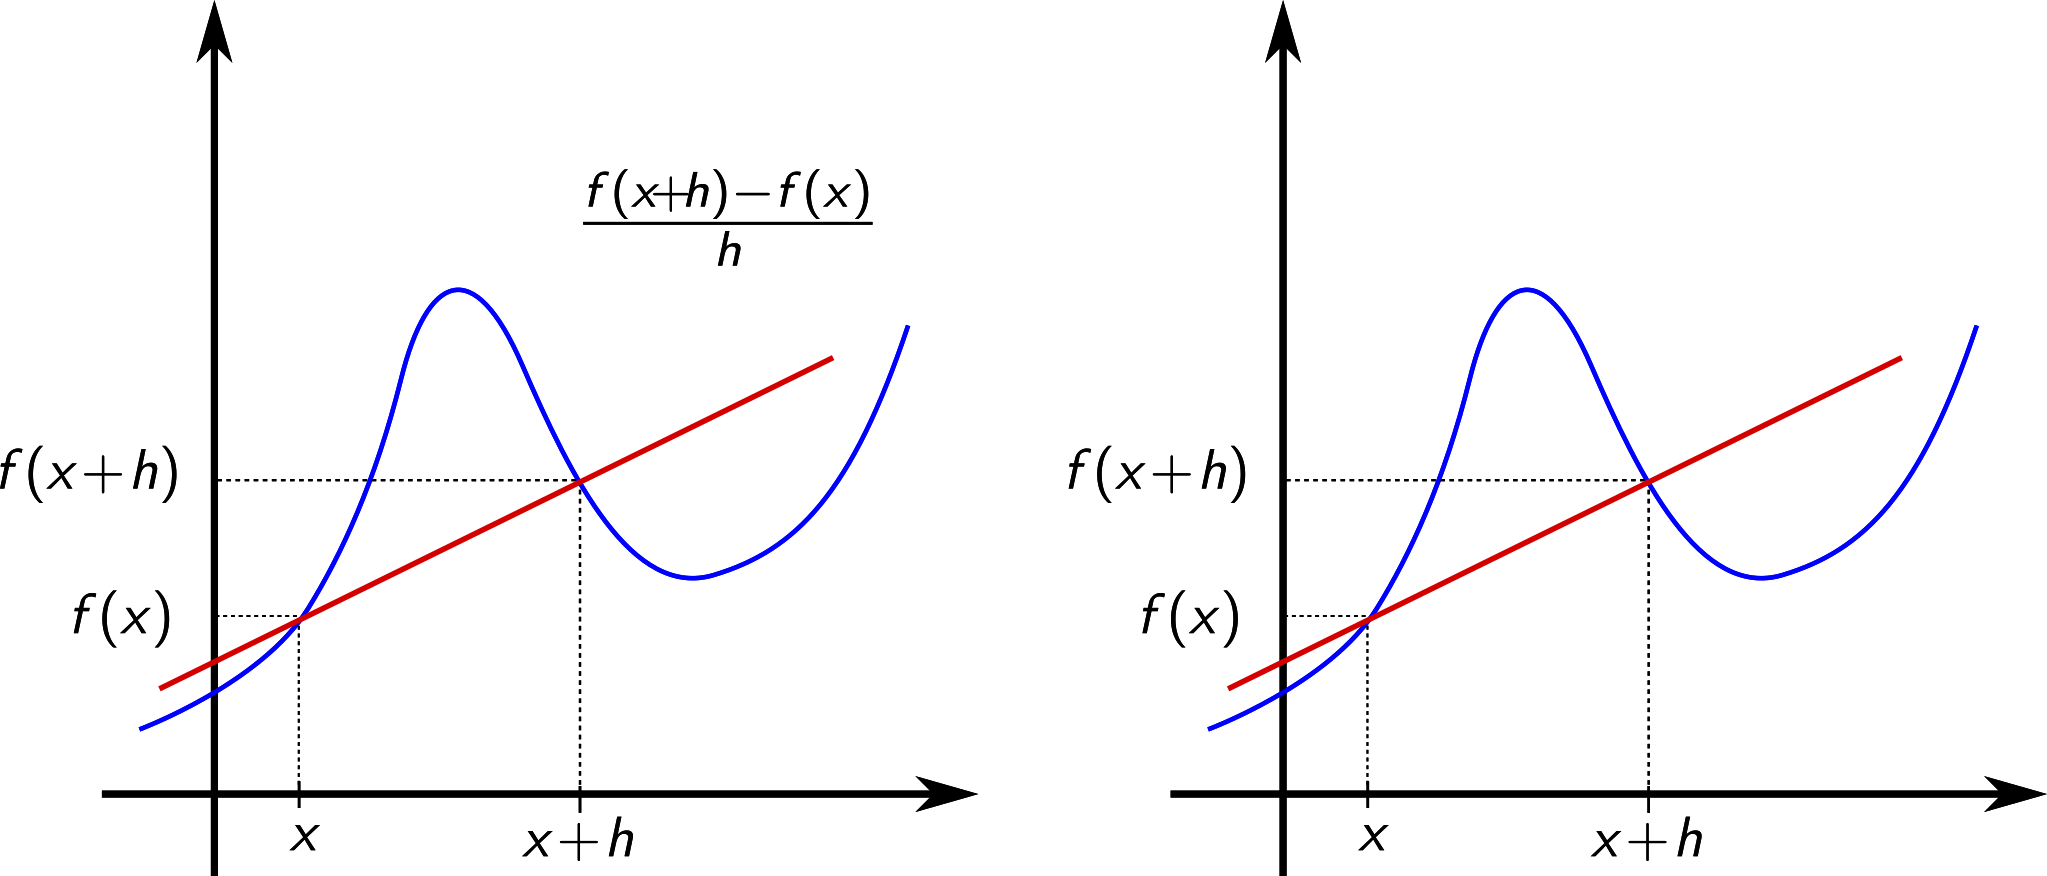
\includegraphics[width=0.9\textwidth]{FIGURES/secant_derivative0}
        \end{center}
        Secant : line joining two point on the graph of $f$. Slope between $(x, f(x))$ and $(x+h, f(x+h))$:
        $$
          \frac{f(x+h)-f(x)}{(x+h)-x} = \frac{f(x+h)-f(x)}{h}
        $$
      \onslide<2>
        \begin{center}
          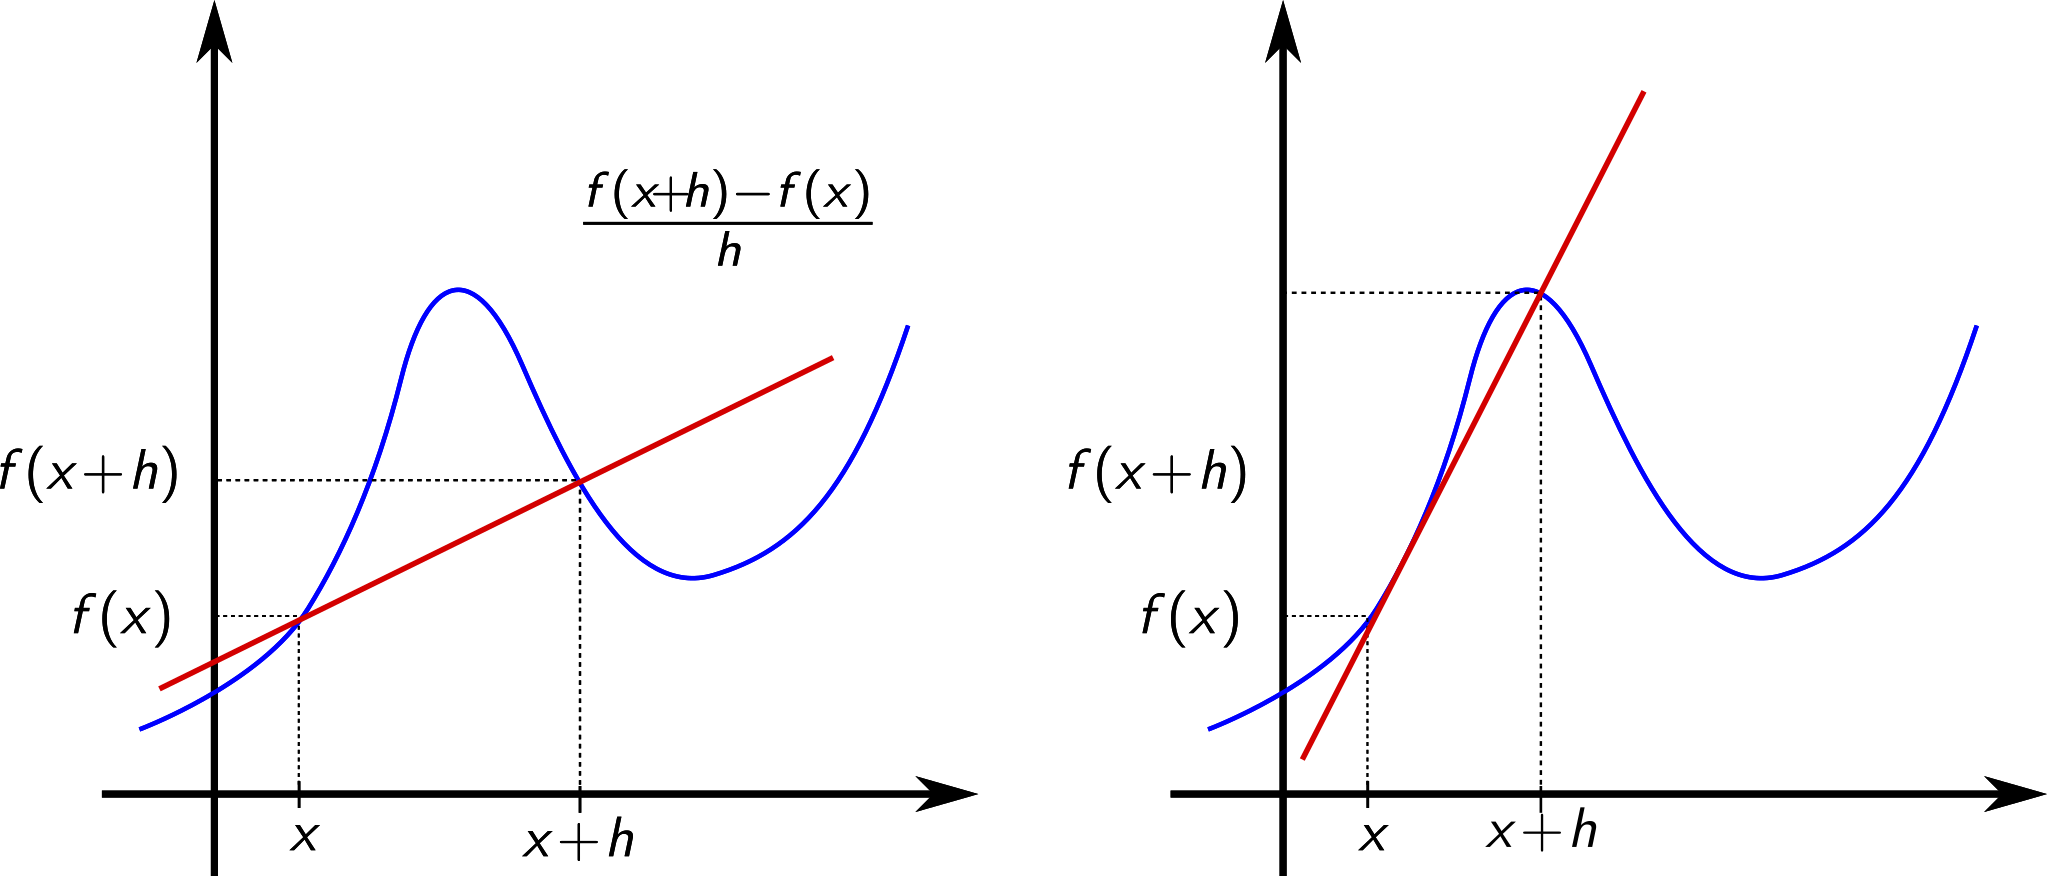
\includegraphics[width=0.9\textwidth]{FIGURES/secant_derivative1}
        \end{center}
      \onslide<3>
        \begin{center}
          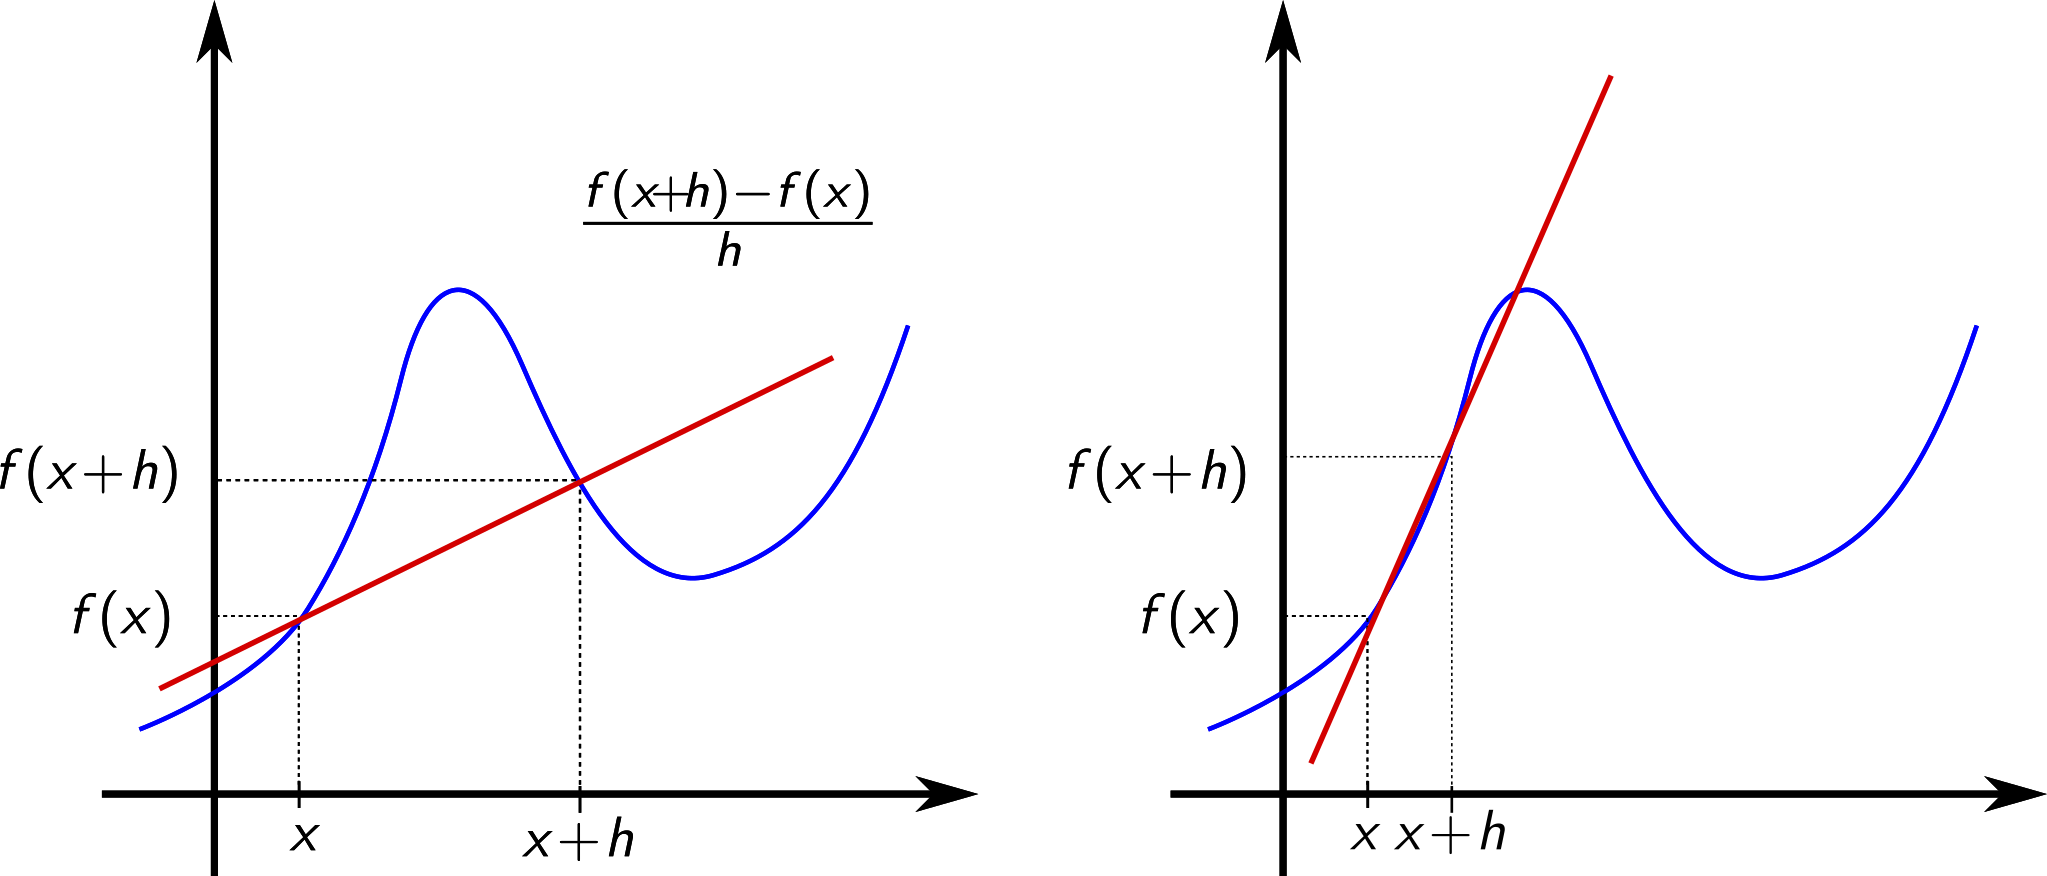
\includegraphics[width=0.9\textwidth]{FIGURES/secant_derivative2}
        \end{center}
        \onslide<4->
        \begin{center}
          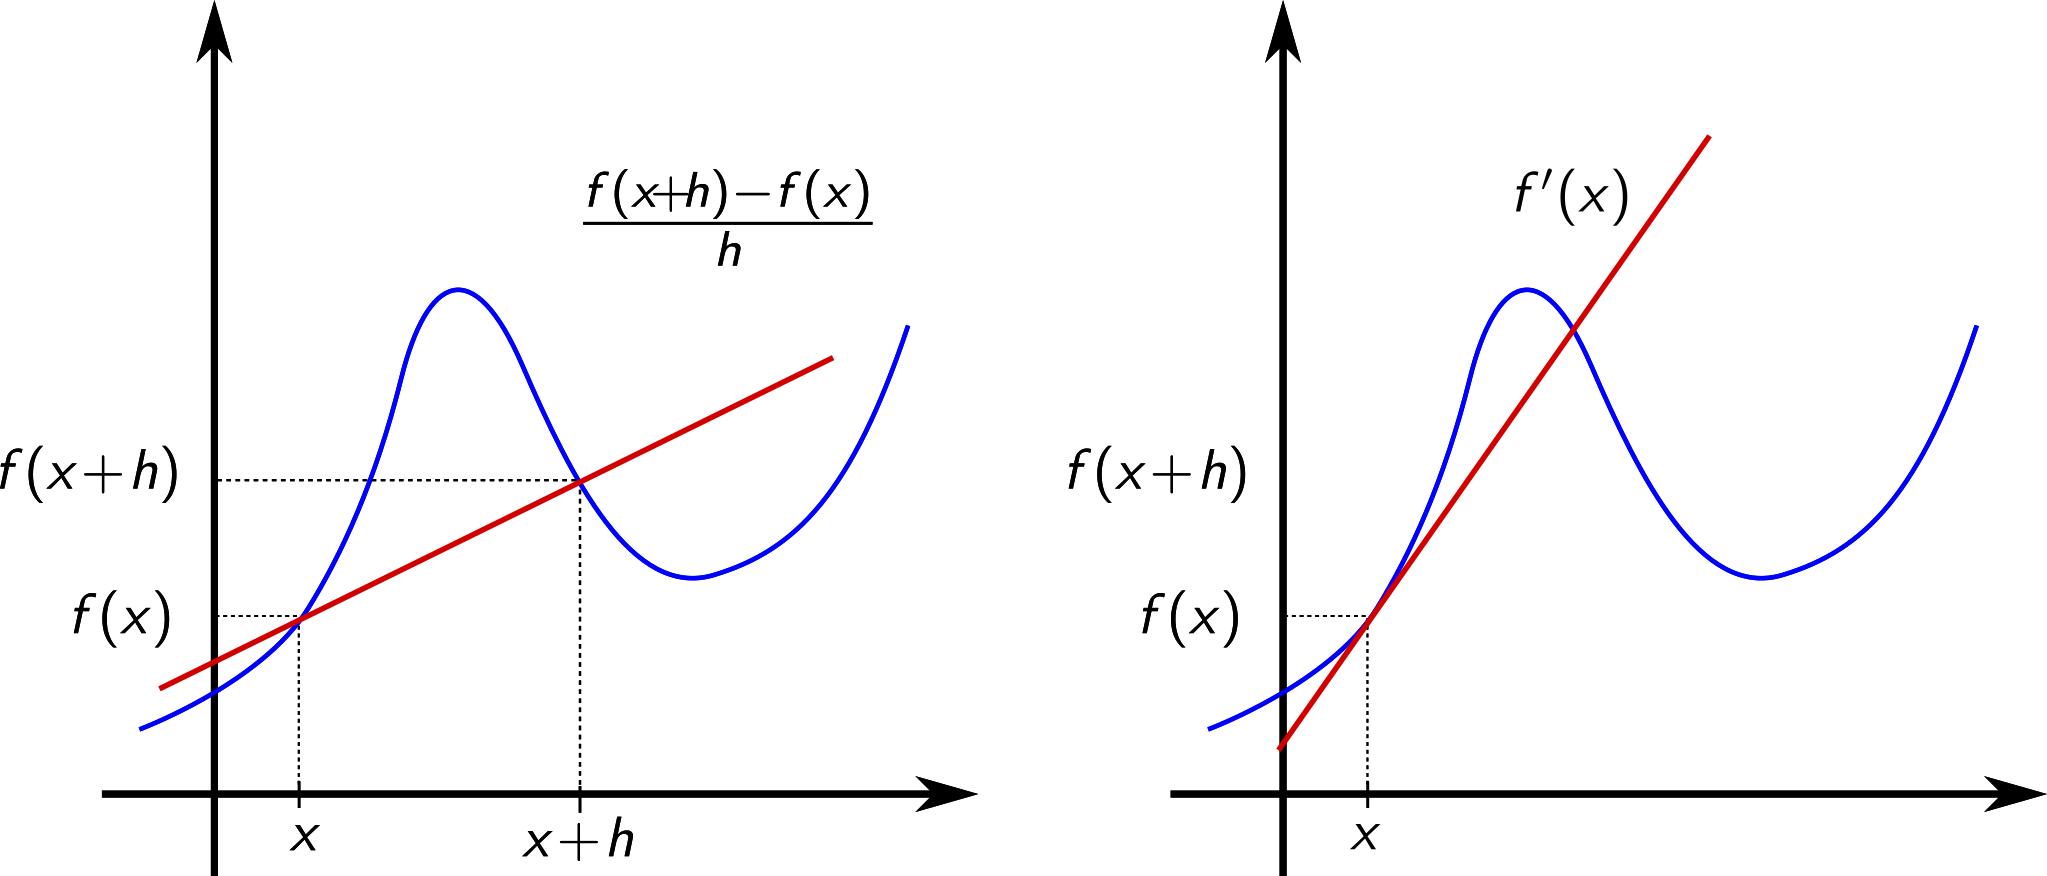
\includegraphics[width=0.9\textwidth]{FIGURES/secant_derivative3}
        \end{center}  
        Derivative: limit of the slope when $h\to 0$ (but $h\not = 0$!) Slope of the tangent at $x$
        $$
          \frac{df}{dx} = f'(x) = \lim_{h\to 0} \frac{f(x+h)-f(x)}{h}
        $$
        \begin{center}
          \fbox{Derivative: a limit on the rate of change of a function.}
        \end{center}
  \end{overprint}
\end{frame}

\begin{frame}{Differentiable function}
  \begin{itemize}
    \item $f$ is \emph{differentiable at $x$} if the limit above exists.
    \item $f$ is \emph{differentiable} if the limit exists for all $x$.
  \end{itemize}
  \pause
  \begin{center}
    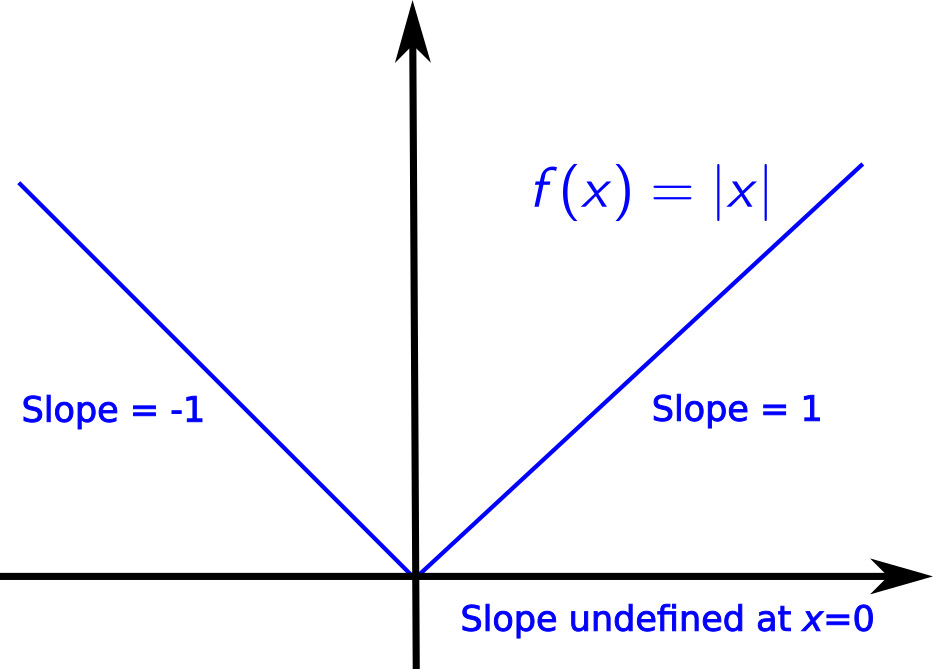
\includegraphics[width=0.5\textwidth]{FIGURES/corner_derivative}
  \end{center}
  \pause
  \begin{itemize}
    \item $f(x) = |x|$ not differentiable at $x=0$.
  \end{itemize}
\end{frame}

\begin{frame}{Derivatives and variations of a function}
  \begin{overprint}
  \onslide<1>
    \begin{center}
      \includegraphics[width=0.4\textwidth]{FIGURES/positive_derivative}\\~\\
      $f'(x) \geq 0$: $f$ is increasing around $x$
    \end{center}
    \onslide<2>
    \begin{center}
      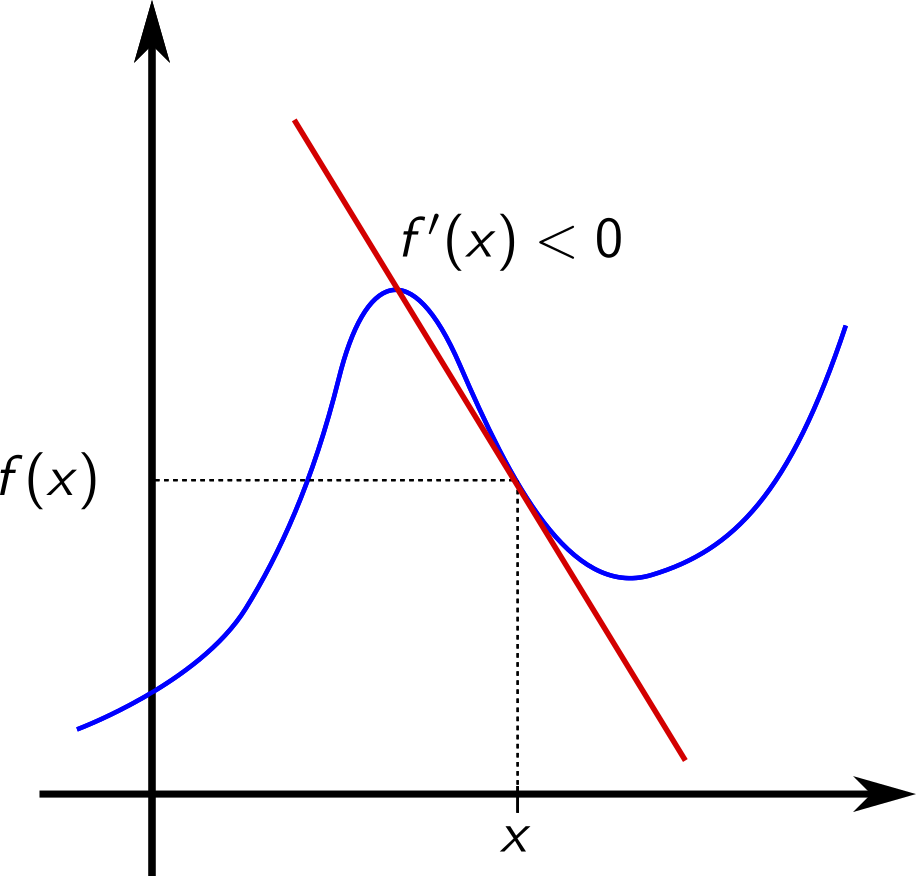
\includegraphics[width=0.4\textwidth]{FIGURES/negative_derivative}\\~\\
      $f'(x) \leq 0$: $f$ is decreasing around $x$
    \end{center}
  \end{overprint}
\end{frame}


\begin{frame}{Null derivative}
  \begin{overprint}
  \onslide<1>
    \begin{center}
      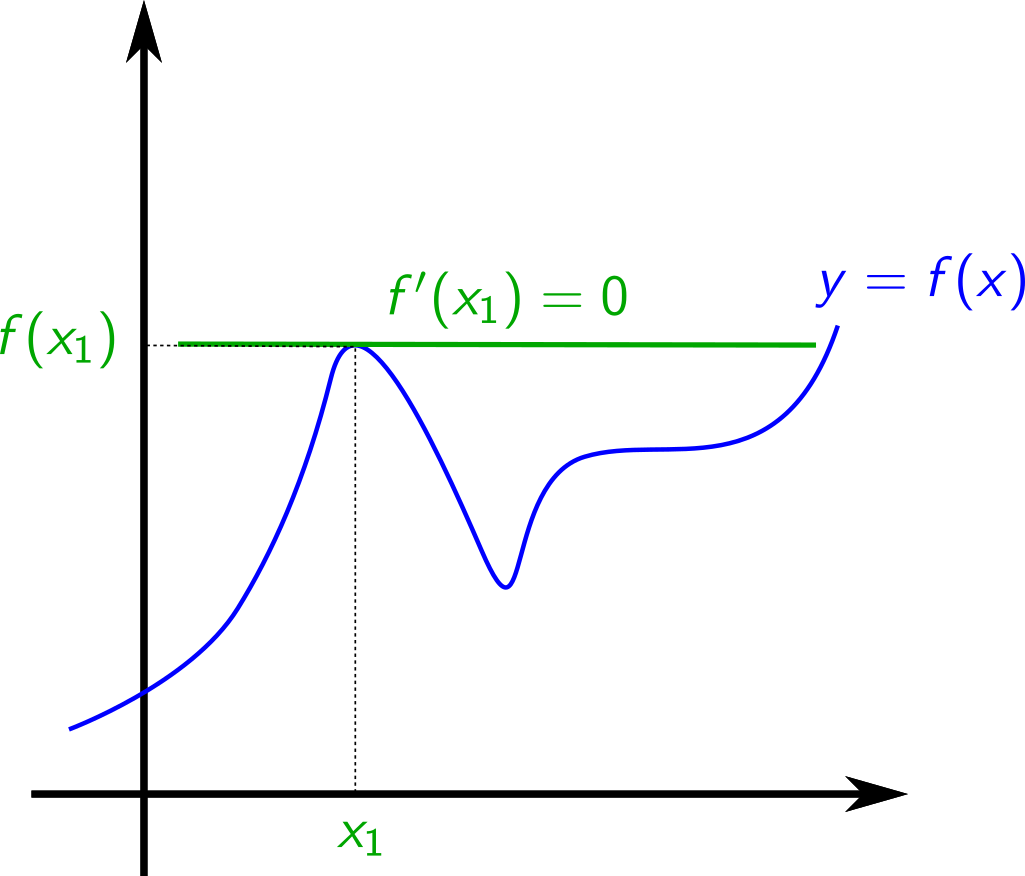
\includegraphics[width=0.4\textwidth]{FIGURES/derivative_at_maximum}
    \end{center}
    \begin{itemize}
      \item $f'(x_1) =0$, $f$ is locally below its tangent: \emph{local maximum}
      \item $f'(x) > 0$ if $x < x_1$ locally, $f'(x) < 0$ if $x>x_1$ locally.
      \item $x_1$ is a \emph{local maximizer} of $f$.
    \end{itemize}
    \onslide<2>
    \begin{center}
      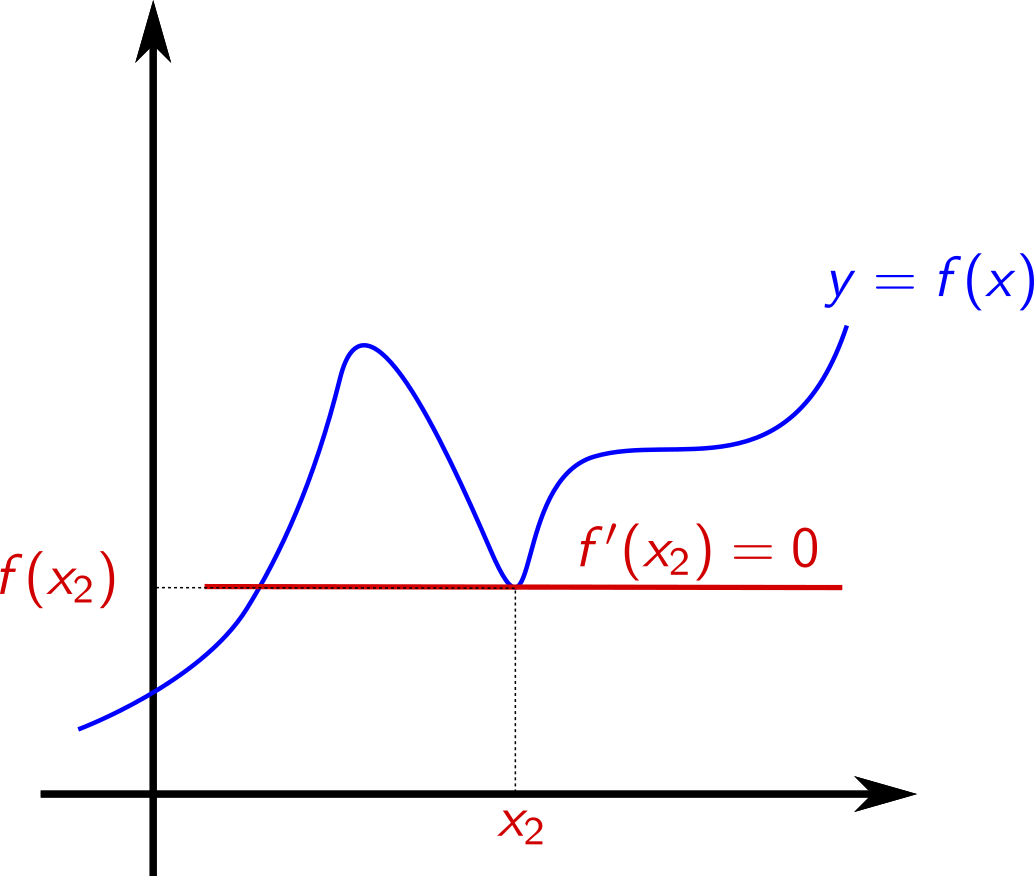
\includegraphics[width=0.4\textwidth]{FIGURES/derivative_at_minimum}\\~\\
    \end{center}
    \begin{itemize}
      \item $f'(x_2) =0$, $f$ is locally above its tangent: \emph{local minimum}
      \item $f'(x) < 0$ if $x < x_2$ locally, $f'(x) < 0$ if $x>x_2$ locally.
      \item $x_2$ is a \emph{local minimizer} of $f$.
    \end{itemize}
    \onslide<3>
    \begin{center}
      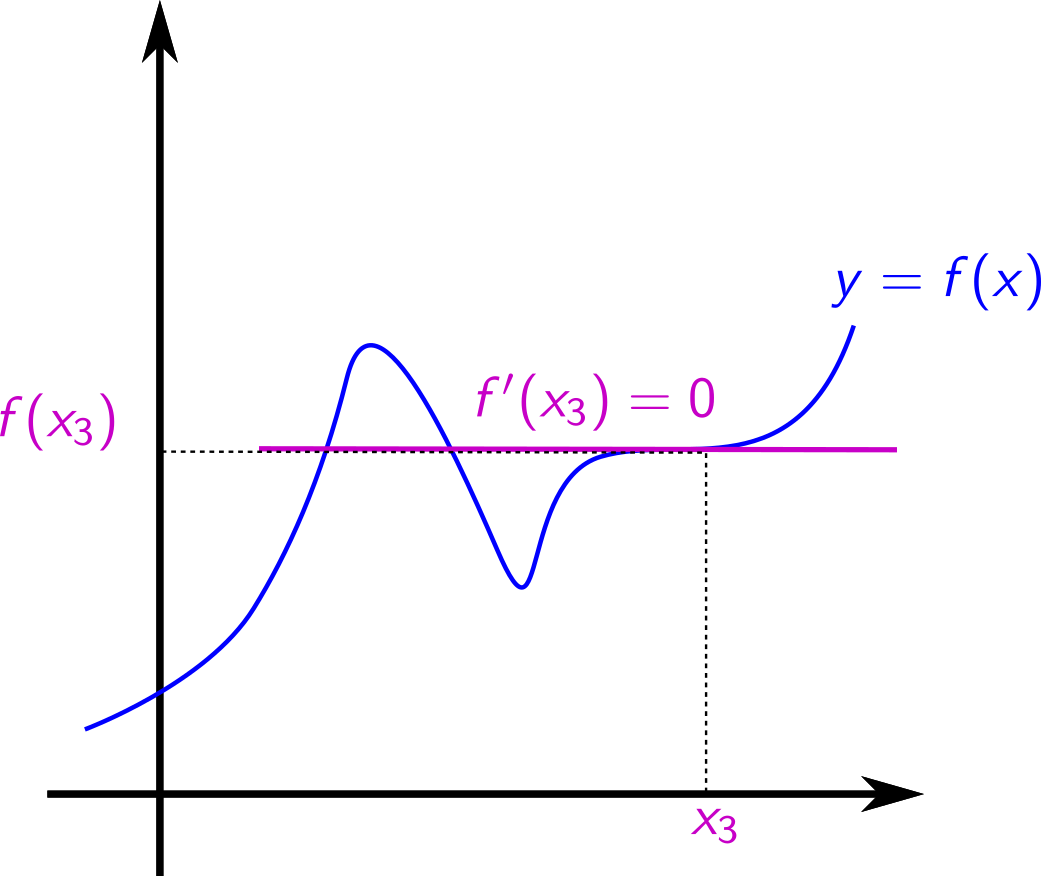
\includegraphics[width=0.4\textwidth]{FIGURES/derivative_at_inflection}
    \end{center}
  \begin{itemize}
    \item $f'(x_3) =0$, $f$ is crosses its tangent. neither minimum nor maximum.
    \item $f'(x) > 0$ if $x < x_3$ locally, $f'(x) > 0$ if $x>x_3$ locally.
    \item $x_3$ is an \emph{inflection point}.
    \item The opposite situation also possible: $f'(x) < 0$ if $x < x_3$ locally, $f'(x) < 0$ if $x>x_3$ locally. Make a picture!
     
  \end{itemize}
  \end{overprint}
\end{frame}

\begin{frame}{Example: Derivative of $x^n$}
  Use the \emph{binomial formula}
  \begin{align*}
    (a + b)^n &= \sum_{k=0}^n {n\choose k}a^{n-k}b^k  \\
    &=a^n + n a^{n-1} b + \frac{n(n-1)}{2}a^{n-2}b^2 + \dots b^n
  \end{align*}
  Develop
  \begin{align*}
    \frac{(x+h)^n - x^n}{h} &= \frac{x^n + h nx^{n-1} + h^2\frac{n(n-1)}{2}x^{n-1} + \dots + h^n - x^n}{h}\\
    &= nx^{n-1} + \udesc{\text{goes }\to 0\text{ when }h\to 0}{h\left(\frac{n(n-1)}{2}x^{n-1} + \dots + h^{n-2}\right)}
  \end{align*}
  The limit when $h\to 0$ is $nx^{n-1}$.
\end{frame}

\begin{frame}{Some Classical Formulas}
\renewcommand{\arraystretch}{1.5}
  \begin{tabular}{|c|c|l|}
    \hline
    function & derivative & domain/remark \\\hline
    $x^\alpha$ & $\alpha x^{\alpha -1}$ & if $\alpha$ is not an integer, $x$ should be $> 0$\\
    \hline
    $e^x$ & $e^x$& $x\in \RR$\\
    \hline
    $\ln x$ &$\frac1x$ & $x > 0$\\
    \hline
    $\sqrt{x}$ & $\frac1{2\sqrt{x}}$ & special case of first rule with $\alpha = \frac12$, $x>0$\\
    \hline
    $\cos x$ & $-\sin x$ &$x\in \RR$\\
    \hline
    $\sin x$ & $\cos x$ & $x\in \RR$\\
    \hline
    $\tan x$ & $\frac1{\cos^2 x}$ &  $x\not= k\pm\frac\pi2,k\in \ZZ$\\
    \hline
    $\arcsin x$ & $\frac1{\sqrt{1-x^2}}$ & $-1<x<1$\\
    \hline
    $\arccos x$ & $-\frac1{\sqrt{1-x^2}}$ & $-1<x<1$\\
    \hline
    $\arctan x$ & $\frac1{1+x^2}$ &$x\in \RR$\\
    \hline
  \end{tabular}
\end{frame}


\begin{frame}{Example: Derivative of a Product -- Leibniz Rule}
  Rule for differentiating $x\mapsto f(x)g(x)$. Write secant ratios:\pause
  \begin{align*}
    \frac{f(x\!+\!h)g(x\!+\!h) - f(x)g(x)}{h} &= \frac{f(x\!+\!h)g(x\!+\!h) - f(x\!+\!h)g(x) + f(x\!+\!h)g(x)-f(x)g(x)}{h}\\
    &= \frac{f(x+h)(g(x+h)-g(x)) + (f(x+h)-f(x))g(x)}{h}\\
    &= f(x+h)\frac{g(x+h)-g(x)}{h} + \frac{f(x+h)-f(x)}{h}g(x)
  \end{align*}
  \pause
  At the limit when $h\to 0$, 
  \begin{itemize}
    \item The first term 
    $$
    f(x+h)\frac{g(x+h)-g(x)}{h} \to f(x)g'(x) 
    $$
    \item The second term 
    $$
    \frac{f(x+h)-f(x)}{h}g(x) \to f'(x)g(x) 
    $$
    \item We get Leibniz Rule: $(f(x)g(x))' = f'(x)g(x) + f(x)g'(x)$.
  \end{itemize}
  
\end{frame}

\begin{frame}{Classical Rules for Computing Derivatives} 
  
\begin{center}
  \begin{tabular}{|c|c|l|}
  \hline
    function & derivative & rule name\\
    \hline
    $\lambda f(x)$ & $\lambda f'(x)$ & scalar multiplication rule\\
    \hline
    $f(x) + g(x)$ & $f'(x) + g'(x)$ & sum rule\\
    \hline
    $f(x)g(x) $ & $f'(x)g(x) + f(x)g'(x)$ & Leibniz rule\\
    \hline
    $\frac{f(x)}{g(x)}$& $\frac{f'(x)g(x)-f(x)g'(x)}{g(x)^2}$ & quotient rule\\
    \hline
    $f(g(x))$ & $f'(g(x)) g'(x)$ & chain rule\\
    \hline
    $e^{f(x)}$ & $f'(x)e^{f(x)}$ & exponentiation rule (chain rule!)\\
    \hline
    $\ln|f(x)|$ & $\frac{f'(x)}{f(x)}$ & logarithm rule \\
    \hline
    $(f(x) g(x))''$ & $f''(x)g(x) + 2f'(x)g'(x) + g''(x)$ & iterated Leibniz rule\\
    \hline
  \end{tabular}
\end{center}
$f''(x)$ is the derivative of $f'(x)$ at $x$. Second (order) derivative of $f$.
\end{frame}

\begin{frame}{A Not That Simple Example: $f(x) = x\cos(e^{\sin(x)})$}
  \begin{itemize}
    \item Write as $f(x) = g(x) h(x)$ with $g(x) = x$, $h(x) = \cos(e^{\sin(x)}) $
    \begin{align*}
      f'(x) &= g'(x)h(x) + g(x)h'(x)&\text{(Leibniz rule)}\\
            &= \cos(e^{\sin(x)}) + x h'(x)& (g'(x) = 1)
    \end{align*}
    \item Write $h(x)$ as $l(m(x))$ with $l(x) = \cos(x)$, $m(x) = e^{\sin(x)}$.
    \begin{align*}
      h'(x) &= l'(m(x)) m'(x) &\text{(chain rule)}\\ 
            &=-\sin(m(x)) m'(x) & (\cos'(x) = -\sin(x))
    \end{align*}
    \item Use Exponential rule $e^{a(x)} = a'(x)e^{a(x)}$ for $m(x) = e^{\sin(x)}$ 
    $$
      \left(e^{\sin(x)}\right)' = \cos(x)e^{\sin(x)},\quad (\sin'(x) = \cos(x)) 
    $$
    \item Reassemble the parts
    $$
      f'(x) = \cos(e^{\sin(x)})  -x\sin(e^{\sin(x)})\cos(x)e^{\sin(x)}
    $$
  \end{itemize}
\end{frame}

\begin{frame}{Example: Arithmetic Mean}
  \begin{itemize}[<+->]
    \item Given $n$ real numbers $x_1,\dots,x_n$.
    \item Classical Arithmetic Mean
    $$
    \bx = \frac1n\sum_{i=1}^n x_i
    $$
  \item Variance function $V(x) = \frac1{2n}\sum_{i=1}^n (x-x_i)^2$. 
  \item When is the derivative 0?
  \begin{align*}
    V'(x) &= \frac1{2n}\sum_{i=1}^n \uder{(x-x_i)^2}{x} = \frac1{2n}\sum_{i=0}^n 2(x-x_i)\\
    & = \frac1n\sum_{i=1}^n (x-x_i) = \frac1n\sum_{i=1}^n x - \frac1n\sum_{i=1}^n x_i\\
    & = x -\bx
  \end{align*}
    \item $V'(x) = 0$ if and only if $x=\bx$. Minimum? Maximum? Inflection point?
    \item Minimum! Why?
    \item The arithmetic mean is the \emph{unique} point where $V(x)$ is minimum!
  \end{itemize}
  
  
\end{frame}

\section{Derivatives in Several Variables}

\begin{frame}{Partial derivatives}
\begin{itemize}
    \item Function $(x,y)\in \RR^2\mapsto f(x,y) \in \RR$: two variables $x$ and $y$.\vfill
    \item partial derivative $\pder{f}{x}(x,y)$ in $x$-direction: derivative of $x\mapsto f(x,y)$. 
    {\small $$
    \pder{f}{x}(x,y)=\lim_{h\to 0} \frac{f(x+h,y)-f(x,y)}{h}
    $$}
    \item partial derivative $\pder{f}{x}(x,y)$ in $y$-direction: derivative of $y\mapsto f(x,y)$
    {\small $$
    \pder{f}{y}(x,y)=\lim_{h\to 0} \frac{f(x,y+h)-f(x,y)}{h}
    $$}
  \end{itemize}
  \begin{columns}
    \begin{column}{0.4\textwidth}
      \begin{center}
        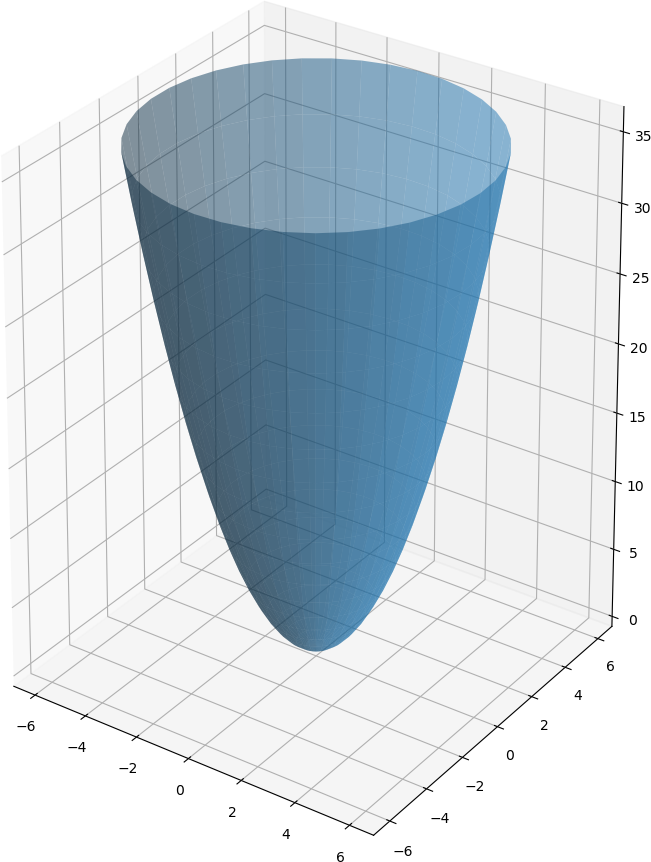
\includegraphics[width=0.8\textwidth]{FIGURES/paraboloid}
      \end{center}
    \end{column}
    \begin{column}{0.7\textwidth}
      \begin{itemize}
        \item if partial derivatives exist at $(x_0,y_0)$ $f$ is \emph{differentiable} at $(x_0,y_0)$.
        \item  if partial derivatives exist everywhere, $f$ is \emph{differentiable}. 
        \item Example $f(x,y)$ = $x^2 + y^2$ (squared Euclidean distance).
        \item Partial derivatives
        $
        \pder{f}{x} = 2x
        $,
        $
        \pder{f}{y} = 2y
        $
        \item $f$ is differentiable.
        \item Euclidean distance: Is $f(x,y) = \sqrt{x^2 + y^2}$ differentiable?
      \end{itemize}
    \end{column}
  \end{columns}
\end{frame}

\begin{frame}{Example $f(x,y) = \frac{xy}{1 + x^2 + y^2}$ }
  \begin{columns}
    \begin{column}{0.6\textwidth}
      \begin{center}
        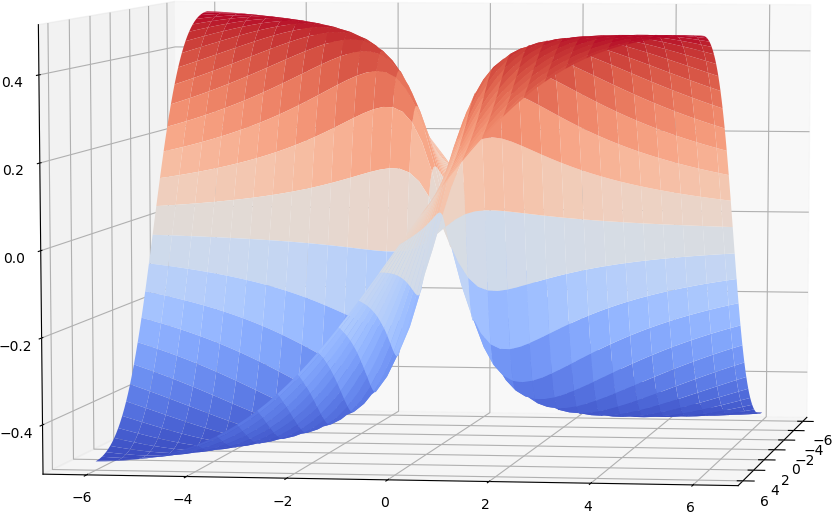
\includegraphics[width=0.7\textwidth]{FIGURES/butterfly_function}
      \end{center}
    \end{column}
    \begin{column}{0.4\textwidth}
      \begin{itemize}
        \item Partial derivatives
        \item in $x$
        $$
        \pder{f}{x} = \frac{y(1-x^2 + y^2)}{(1 + x^2+y^2)^2}
        $$
        \item in $y$
        $$ 
        \pder{f}{x} = \frac{x(1+x^2 - y^2)}{(1 + x^2+y^2)^2}
        $$
      \end{itemize}
    \end{column}
  \end{columns}
  \medskip
  \begin{itemize}
    \item Computation in $x$. $y$ supposed to be fixed: Using quotient rule, power rule, 
    \begin{align*}
      \pder{f}{x}(x,y) & = \frac{
      \pder{xy}{x}(1+x^2+y^2) - xy\pder{(1+x^2+y^2)}{x}}{(1+x^2+y^2)^2}\\
      &= \frac{y(1+x^2+y^2) -xy(2x)}{(1+x^2+y^2)^2}= \frac{y(1-x^2+y^2)}{(1+x^2+y^2)^2}
    \end{align*}
  \end{itemize}
\end{frame}


\begin{frame}{Differential, Gradient}
  \begin{itemize}[<+->]
    \item Differential of $f(x,y)$: the \emph{line vector} made of partial derivatives.
    $$
    Df(x,y) = \left(\pder{f}{x},\pder{f}{y}\right)
    $$\vfill
    \item Gradient of $f(x,y)$: the \emph{column vector} made of partial derivatives.
    $$
    \nabla f(x,y) = \begin{bmatrix}\pder{f}{x}\\\pder{f}{y}\end{bmatrix} = Df(x,y)^T
    $$\vfill
    \item Difference between Differential and Gradient:  not too much \emph{in this course!}
    \vfill
    \item[\raisebox{1mm}{\dbend}] $Df(x,y)^TDf(x,y)$ is a matrix, $\nabla f(x,y)^T \nabla f(x,y)$ is a real (Linear Algebra) 
    \vfill
    \item $\nabla f(x,y)^T \nabla f(x,y) = \|\nabla f(x,y)\|^2$ : length of gradient vector.
  \end{itemize}
\end{frame}

\begin{frame}{Gradients and Critical Points}
  \begin{itemize}
    \item A point $(x,y)$ is \emph{critical} for $f$ if $\nabla f(x,y) = \vec{0}$. Minima, Maxima, Saddle points...
  \end{itemize}
  \begin{center}
  {\small
  \begin{tabular}{ccc}
    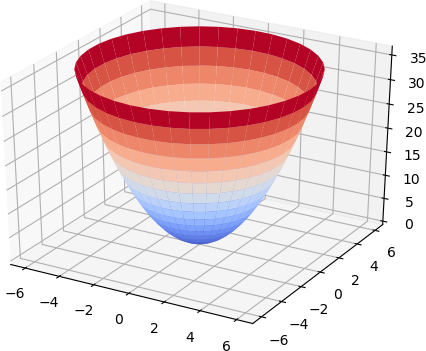
\includegraphics[width=0.25\textwidth]{FIGURES/paraboloid2} &
    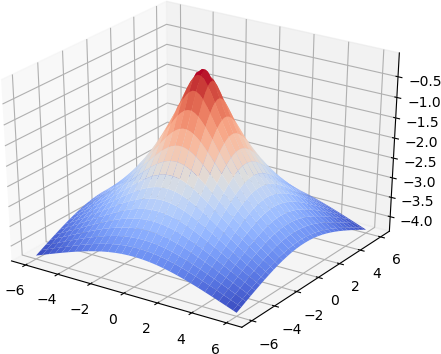
\includegraphics[width=0.25\textwidth]{FIGURES/logstuff} &
    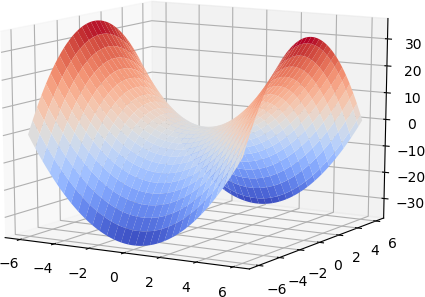
\includegraphics[width=0.25\textwidth]{FIGURES/Saddle}\\
    $f(x,y)=x^2+y^2$ & $g(x,y) = -\log(1\!+\!x^2\!+\!y^2)$ & $h(x,y) = x^2-y^2$
  \end{tabular}
  }
  \end{center}
  \begin{itemize}
    \item All the three functions have only one critical point, at $(x,y) = (0,0)$.
    \item For $f$: minimum
    \item For $g$: maximum
    \item For $h$: saddle point.
  \end{itemize}
\end{frame}

\begin{frame} \frametitle{Gradients and Optimization}

\uncover<2->{{\bf Fact:} The gradient points in the direction of the steepest ascent of the function.
\uncover<3->{Its opposite points in the direction of steepest descent.}
\vspace{-0.2cm}
\begin{figure}
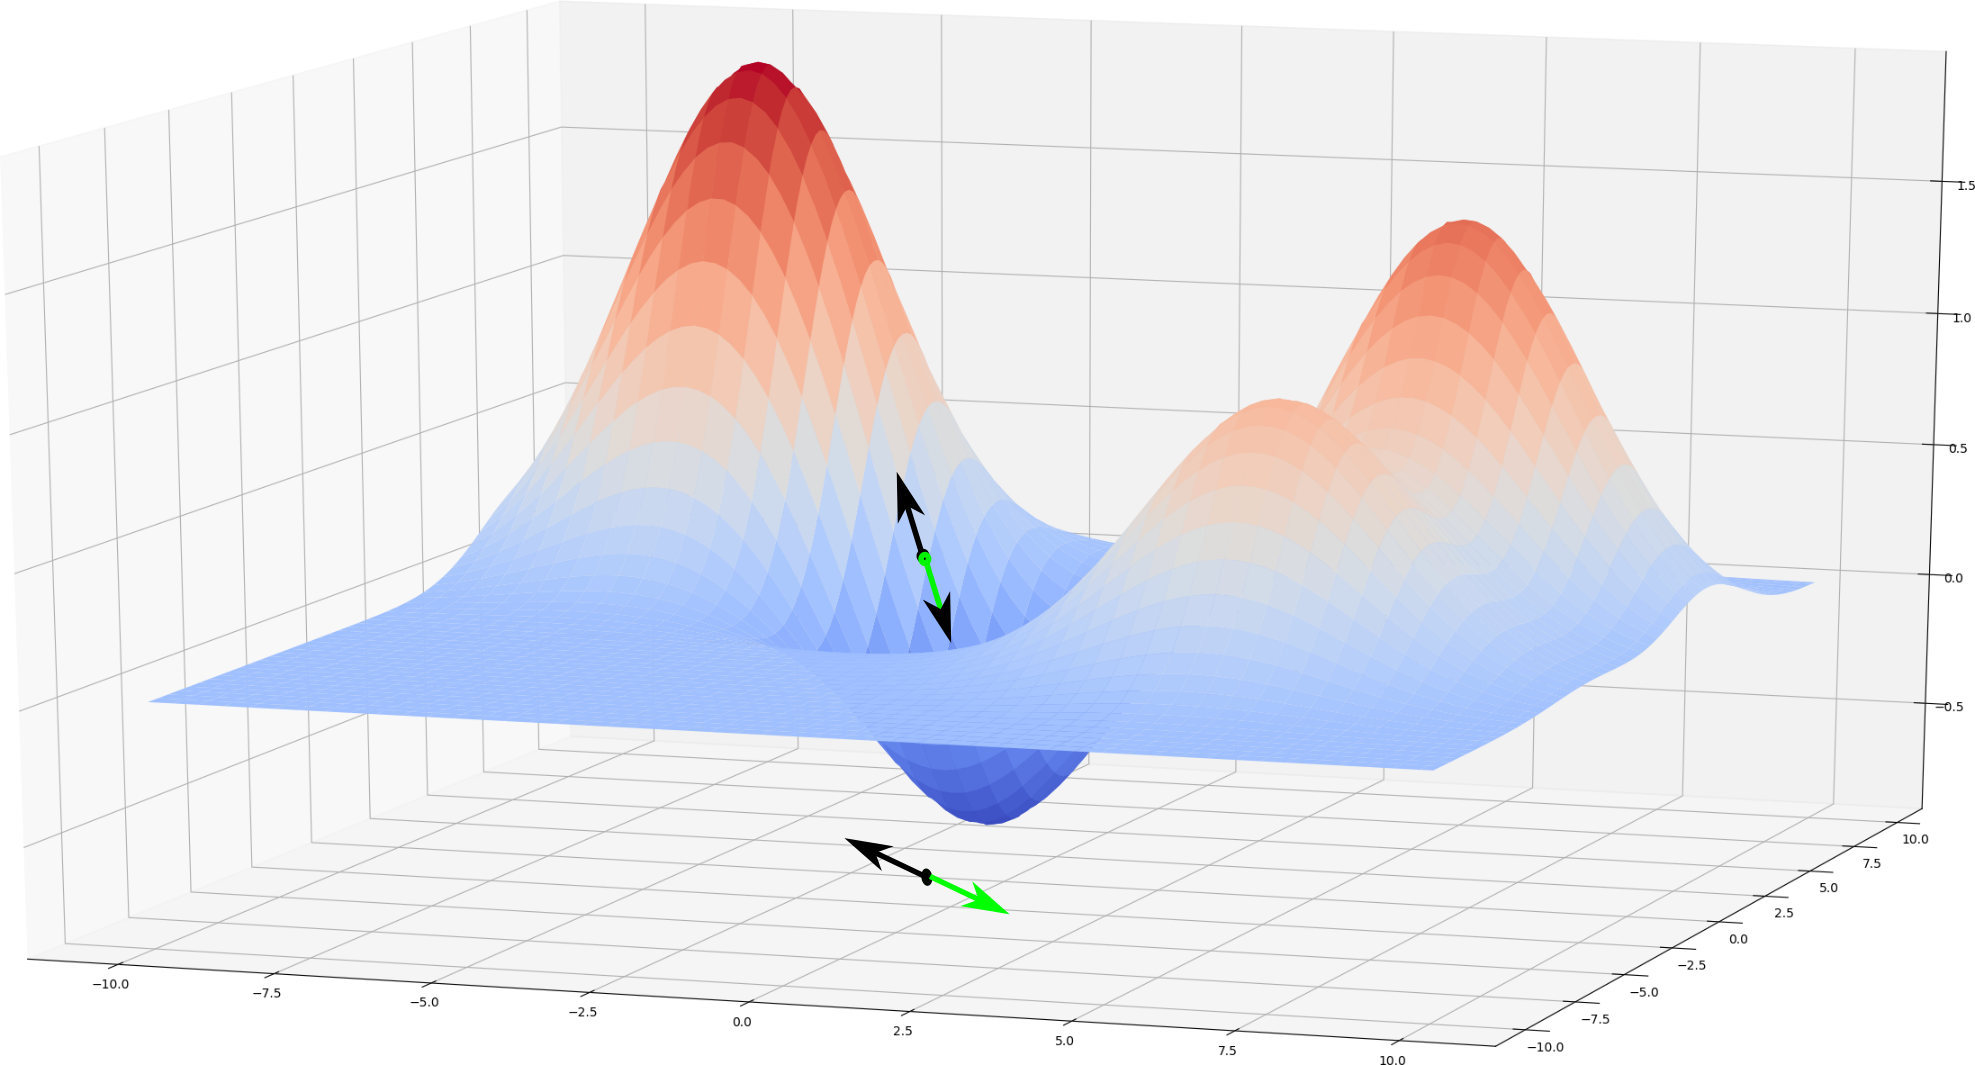
\includegraphics[width=0.7\linewidth]{FIGURES/bumpfn_annotated}
\end{figure}
}
\uncover<4->{
What can this be useful for? \uncover<5->{{\bf Optimization -- gradient descent!}}
}
\end{frame}




\begin{frame}{Second order derivatives}
  \begin{itemize}
    \item Second order derivatives in $x$: Different combinations 
    $$
    \pderd{2}{f}{x^2} = \pder{}{x}\pder{f}{x}, \quad \pderd{2}{f}{y^2}=\pder{}{y}\pder{f}{y}
    $$
    \item \emph{Mixed} Partial Derivatives: (equality from Schwarz' Theorem)
    $$
    \pderd{2}{f}{xy} = \pder{}{x}\pder{f}{y} = \pder{}{y}\pder{f}{x} = \pderd{2}{f}{yx}
    $$
    \item \emph{Hessian matrix} of $f$: \emph{symmetric} matrix (still function of $x$ and $y$)
    $$
    \Hess f = \begin{bmatrix}
      \pderd{2}{f}{x^2} & \pderd{2}{f}{xy}\\
      \pderd{2}{f}{xy} & \pderd{2}{f}{y^2}
    \end{bmatrix}
    $$
    \item \emph{Laplacian} of $f$: 
    $$
    \Delta f = \pderd{2}{f}{x^2} + \pderd{2}{f}{y^2} = \text{Trace} \Hess f
    $$
  \end{itemize}
\end{frame}

\begin{frame}{Some Examples}
\begin{itemize}
  \item Hessian of $f(x,y) = x^2 + y^2$
  $$
  \Hess f = \begin{bmatrix}
    2 & 0\\
    0 & 2
  \end{bmatrix} = 2 I_2,\quad I_2 = 2\times 2\text{-identity matrix}
  $$
  \item $\Delta f = 4$.\vfill
  \item Hessian of $f(x,y) = \frac{xy}{1+x^2+y^2}$: not as nice as previous one!
  $$
  \Hess f = \frac{1}{(x^2+y^2+1)^3}
  \begin{bmatrix}
 2 x y \left(x^2-3 y^2-3\right) & 6 x^2 y^2-x^4-y^4+1 \\
 6 x^2 y^2-x^4-y^4+1 & -2 x y \left(3 x^2-y^2+3\right) 
  \end{bmatrix}
  $$
  \item Laplacian of $f$
  $$
  \Delta f = -\frac{4 x y \left(x^2+y^2+3\right)}{\left(x^2+y^2+1\right)^3}
  $$
\end{itemize}
\end{frame}


\begin{frame}{In More Variables}
Function $f(x_1,x_2,\dots,x_n):\RR^n\to \RR$.
\begin{itemize}
\item Partial Derivative w.r.t $x_i$
$$
\pder{f}{x_i} = \lim_{h\to 0}\frac{f(x_1,x_2,\dots,x_{i-1},x_i+h,x_{i+1},\dots x_n) - f(x_1,x_2,\dots,x_{i-1},x_i,x_{i+1},\dots x_n)}{h}
$$
\item The same, but we need more letters!
\item Differentials, Gradients:
  $$
  Df = \left(\pder{f}{x_1},\dots,\pder{f}{x_n}\right),\quad \nabla f = \left(\pder{f}{x_1},\dots,\pder{f}{x_n}\right)^T
  $$
  \item Hessian: $n\times n$ symmetric matrices
  $$
  \Hess f = 
   \begin{bmatrix}
     \pderd{2}{f}{x_1^2} & \pderd{2}{f}{x_1x_2} & \dots & \pderd{2}{f}{x_1x_n}\\
     \pderd{2}{f}{x_1x_2} & \pderd{2}{f}{x_2^2} & \dots & \pderd{2}{f}{x_2x_n}\\
     \vdots & \vdots & & \vdots\\
     \pderd{2}{f}{x_1x_n} & \pderd{2}{f}{x_2x_n} & \dots & \pderd{2}{f}{x_n^2}
   \end{bmatrix}
  $$
  \item Laplacian
    $$
    \nabla f = \sum_{i=1}^n \pderd{2}{f}{x^i}
    $$
\end{itemize}  
\end{frame}



\begin{frame}
\vfill
\begin{center}
  \Huge That's all Folk!
\end{center}
\vfill  
\end{frame}

\end{document}
